% Visão geral do experimento, versão de uma coluna (figura do paper). Compilar: pdflatex overview.tex -> overview.pdf
% Versão larga, com mais detalhes: overview_detalhada.tex
\documentclass[tikz,border=1pt]{standalone}
\usepackage[T1]{fontenc}
\usepackage[utf8]{inputenc}
\usepackage{libertine}
\usetikzlibrary{positioning,arrows.meta}
\definecolor{tinta}{HTML}{3B2A20}
\definecolor{ga}{HTML}{6B4430}
\definecolor{gb}{HTML}{8A6C55}
\definecolor{gc}{HTML}{5E6849}
\begin{document}
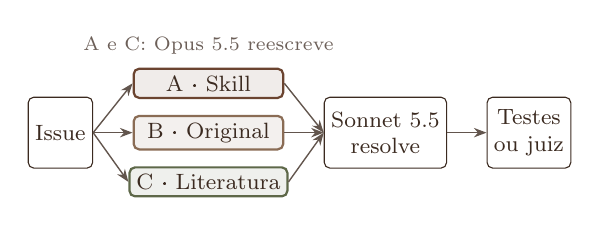
\begin{tikzpicture}[
  font=\footnotesize, text=tinta, node distance=2mm and 5mm,
  caixa/.style={draw=tinta, rounded corners=2pt, align=center, inner sep=2.5pt, minimum height=9mm},
  grupo/.style={draw=#1, line width=0.8pt, fill=#1!10, rounded corners=2pt, align=center, inner sep=2.5pt, minimum width=19mm},
  nota/.style={font=\scriptsize, text=tinta!75},
  seta/.style={-{Stealth[length=1.6mm]}, draw=tinta!80, line width=0.5pt}]
\node[grupo=gb] (b) {B · Original};
\node[grupo=ga, above=of b] (a) {A · Skill};
\node[grupo=gc, below=of b] (c) {C · Literatura};
\node[caixa, left=of b] (issue) {Issue};
\node[caixa, right=of b] (res) {Sonnet 5.5\\resolve};
\node[caixa, right=of res] (aval) {Testes\\ou juiz};
\foreach \g in {a,b,c} {\draw[seta] (issue.east) -- (\g.west); \draw[seta] (\g.east) -- (res.west);}
\draw[seta] (res) -- (aval);
\node[nota, above=0.5mm of a] {A e C: Opus 5.5 reescreve};
\end{tikzpicture}
\end{document}
